\section{Closed-loop results and compute}\label{sec:closedloop}

\subsection{Safety and recovery}
Table~\ref{tab:closedloop} reports 400 fresh CSTR episodes per model, with every policy run on the same episodes.
Validating every proposal recovers 34--54\% of episodes. Never validating executes a failing action in 64--80\% of
episodes, and random routing at the screens' skip rates executes 107--186 failing actions (except for Llama-3.2-3B,
whose random policy, like its probes, never accepted). The trained screens execute far fewer failing actions while
avoiding 29--90\% of validator calls. On first proposals they behave as they did offline: the observable screen
executed 0--13 failing actions unchecked per 400 episodes.

\paragraph{Retries are a distribution shift for internal signals} For two models, probes that use internal signals
accepted many failing \emph{retries}: the combined probe of Qwen2.5-7B executed 165 failing actions, 161 of them on
retries, and SmolLM2's combined and internals-only probes executed 237 and 243, nearly all on retries. The probes were
trained on first proposals. A retry prompt contains the validator's failure feedback, which shifts the model's
internal state, and the probes misread failing retries as safe. Observable-only probes, whose inputs do not change
between first proposals and retries, were unaffected.

\paragraph{The first-proposal-only rule} Allowing unchecked execution only for first proposals (R0) and validating
every retry removes these failures (Table~\ref{tab:closedloop}). For SmolLM2, failing executions fell from 237 to 11
(combined) and from 243 to 2 (internals only), with recovery unchanged ($-1.0$ [$-2.0$, $-0.3$] and $-0.5$ [$-1.3$,
0.0] points relative to always-validate) and validator calls still reduced by 65\% and 42\%. For Qwen2.5-7B the
combined probe's failing executions fell from 165 to 4, with recovery unchanged within uncertainty
($-1.5$ [$-4.5$, $+1.5$] points) and validator calls still reduced by 41\%. For the other three
models the rule changes nothing, because their probes accepted no failing retries. With R0, an internals-only screen,
which uses no plant measurements and no model of the plant, avoided 29--65\% of validator calls across the five models
while executing 0--2 failing actions unchecked.

\paragraph{Where recovery is lost} The screens' recovery cost ranges from $-0.5$ to $-18.5$ points. It comes from
unchecked \emph{rejects}, not from unsafe accepts: each reject requires a new proposal and consumes the six-proposal
budget, and some rejected proposals were good (up to 0.45 per episode for Qwen2.5-3B's internals-only screen). For
Llama-3.2-3B, whose proposals rarely pass, every skipped call is a reject, and recovery falls by 4.0 (internals only)
to 18.5 (observables) points. For the two smallest models, validation itself does not improve recovery
(never-validate recovers as often as always-validate) because they mostly repeat their proposals; there, validation
and the screens serve to prevent the execution of failing actions.

\begin{table*}[t]
\centering
\small
\caption{Closed-loop CSTR recovery on 400 fresh episodes per model. $\Delta$: paired difference to always-validate (percentage points, bootstrap 95\% CI over episodes). Unsafe: failing actions executed without validation. Calls: validator calls avoided relative to always-validate. R0: the probe may skip validation only for first proposals (retries are always validated).}
\label{tab:closedloop}
\begin{tabular}{llrrrr}
\toprule
Model & Policy & Recovered (\%) & $\Delta$ recovered & Unsafe & Calls avoided \\
\midrule
Qwen-1.5B & Always validate & 34.5 & -- & 0 & -- \\
 & Observables & 33.0 & -1.5 [-3.0, -0.2] & 12 & 67\% \\
 & Obs.+int.+grd. & 33.2 & -1.2 [-2.5, +0.0] & 9 & 64\% \\
 & Internals only & 33.2 & -1.2 [-2.5, -0.2] & 0 & 35\% \\
 & Random (matched) & 33.8 & -0.8 [-1.8, +0.0] & 186 & 60\% \\
 & Never validate & 34.5 & +0.0 [+0.0, +0.0] & 259 & 100\% \\
\midrule
Qwen-3B & Always validate & 43.8 & -- & 0 & -- \\
 & Observables & 41.0 & -2.8 [-5.8, +0.2] & 0 & 47\% \\
 & Obs.+int.+grd. & 37.0 & -6.8 [-10.2, -3.5] & 1 & 72\% \\
 & Internals only & 30.0 & -13.8 [-17.5, -10.5] & 0 & 65\% \\
 & Random (matched) & 37.8 & -6.0 [-9.0, -3.0] & 110 & 47\% \\
 & Never validate & 30.0 & -13.8 [-17.2, -10.5] & 274 & 100\% \\
\midrule
Qwen-7B & Always validate & 0.0 & -- & 0 & -- \\
 & Observables & 0.0 & +0.0 [+0.0, +0.0] & 1 & 60\% \\
 & Observables, R0 & 0.0 & +0.0 [+0.0, +0.0] & 0 & 20\% \\
 & Obs.+int.+grd. & 0.0 & +0.0 [+0.0, +0.0] & 1 & 80\% \\
 & Obs.+int.+grd., R0 & 0.0 & +0.0 [+0.0, +0.0] & 0 & 20\% \\
 & Internals only & 0.0 & +0.0 [+0.0, +0.0] & 0 & 20\% \\
 & Internals only, R0 & 0.0 & +0.0 [+0.0, +0.0] & 0 & 20\% \\
 & Random (matched) & 0.0 & +0.0 [+0.0, +0.0] & 1 & 40\% \\
 & Never validate & 0.0 & +0.0 [+0.0, +0.0] & 2 & 100\% \\
\midrule
Llama-3B & Always validate & 53.8 & -- & 0 & -- \\
 & Observables & 35.2 & -18.5 [-23.5, -13.2] & 0 & 62\% \\
 & Obs.+int.+grd. & 44.5 & -9.2 [-13.8, -4.5] & 0 & 45\% \\
 & Internals only & 49.8 & -4.0 [-8.0, +0.0] & 0 & 29\% \\
 & Random (matched) & 29.5 & -24.2 [-29.2, -19.0] & 0 & 68\% \\
 & Never validate & 15.2 & -38.5 [-43.2, -33.8] & 312 & 100\% \\
\midrule
SmolLM-1.7B & Always validate & 36.5 & -- & 0 & -- \\
 & Observables & 35.2 & -1.2 [-2.5, -0.2] & 13 & 62\% \\
 & Observables, R0 & 35.2 & -1.2 [-2.5, -0.2] & 13 & 62\% \\
 & Obs.+int.+grd. & 35.0 & -1.5 [-2.8, -0.5] & 237 & 66\% \\
 & Obs.+int.+grd., R0 & 35.5 & -1.0 [-2.0, -0.2] & 11 & 65\% \\
 & Internals only & 35.5 & -1.0 [-2.0, -0.2] & 243 & 44\% \\
 & Internals only, R0 & 36.0 & -0.5 [-1.2, +0.0] & 2 & 42\% \\
 & Random (matched) & 34.0 & -2.5 [-4.2, -1.0] & 172 & 65\% \\
 & Never validate & 36.0 & -0.5 [-1.2, +0.0] & 254 & 100\% \\
\bottomrule
\end{tabular}
\end{table*}


\subsection{Compute}
Generation dominates the per-episode compute on our hardware (Table~\ref{tab:costs}); the feature passes needed by
internal signals add 2--14\,s per episode (the most for Llama-3.2-3B). At the measured validator cost (7.8--11.6\,s per call), the screens save
little or cost time, because every unchecked reject triggers a regeneration that costs about as much as the
validation it replaces. The screen's cost, however, is independent of the simulator, while the validator's cost grows
with the simulated horizon, model fidelity and number of scenarios. Re-costing the same decisions
(Fig.~\ref{fig:costs}) shows savings of 11--49\% of total compute at 30\,s per validation and
21--64\% at 60\,s for four of the five models, with break-even validator costs of 2--18\,s. Llama-3.2-3B is
the exception: since it is screened only by rejection, its break-even lies above 70\,s, and its timings are
additionally inflated by GPU memory pressure in our runs.

\begin{table*}[t]
\centering
\small
\caption{Compute per episode relative to always-validate (positive = saving). The logged closed-loop decisions do not depend on validator latency (the plant is paused during decisions), so the same decisions are re-costed exactly for a validator taking 30\,s or 60\,s per call. Break-even: validator cost per call above which the policy saves time.}
\label{tab:costs}
\begin{tabular}{llrrrr}
\toprule
Model & Policy & Measured & 30\,s & 60\,s & Break-even (s) \\
\midrule
Qwen-1.5B & Observables probe & +11\% & +28\% & +40\% & 3 \\
 & Obs. + internals + grounding probe & +5\% & +23\% & +36\% & 7 \\
 & Internals-only probe & +6\% & +14\% & +21\% & 3 \\
\midrule
Qwen-3B & Observables probe & +2\% & +21\% & +30\% & 7 \\
 & Obs. + internals + grounding probe & -4\% & +28\% & +44\% & 10 \\
 & Internals-only probe & -19\% & +16\% & +34\% & 17 \\
\midrule
Llama-3B & Observables probe & -40\% & -22\% & -5\% & 73 \\
 & Obs. + internals + grounding probe & -40\% & -24\% & -11\% & 97 \\
 & Internals-only probe & -29\% & -18\% & -9\% & 107 \\
\midrule
Qwen-7B & Observables probe & +18\% & +49\% & +64\% & 2 \\
 & Observables probe, first-proposal-only & +17\% & +47\% & +62\% & 3 \\
 & Obs. + internals + grounding probe & +31\% & +50\% & +59\% & any \\
 & Obs. + internals + grounding, first-proposal-only & -1\% & +17\% & +26\% & 9 \\
 & Internals-only probe & -1\% & +18\% & +28\% & 9 \\
 & Internals-only, first-proposal-only & -2\% & +17\% & +27\% & 10 \\
\midrule
SmolLM-1.7B & Observables probe & +0\% & +24\% & +39\% & 12 \\
 & Observables probe, first-proposal-only & -7\% & +20\% & +36\% & 15 \\
 & Obs. + internals + grounding probe & +44\% & +52\% & +58\% & any \\
 & Obs. + internals + grounding, first-proposal-only & -1\% & +25\% & +41\% & 12 \\
 & Internals-only probe & +40\% & +42\% & +43\% & any \\
 & Internals-only, first-proposal-only & -9\% & +11\% & +23\% & 18 \\
\bottomrule
\end{tabular}
\end{table*}


\begin{figure}[t]
\centering
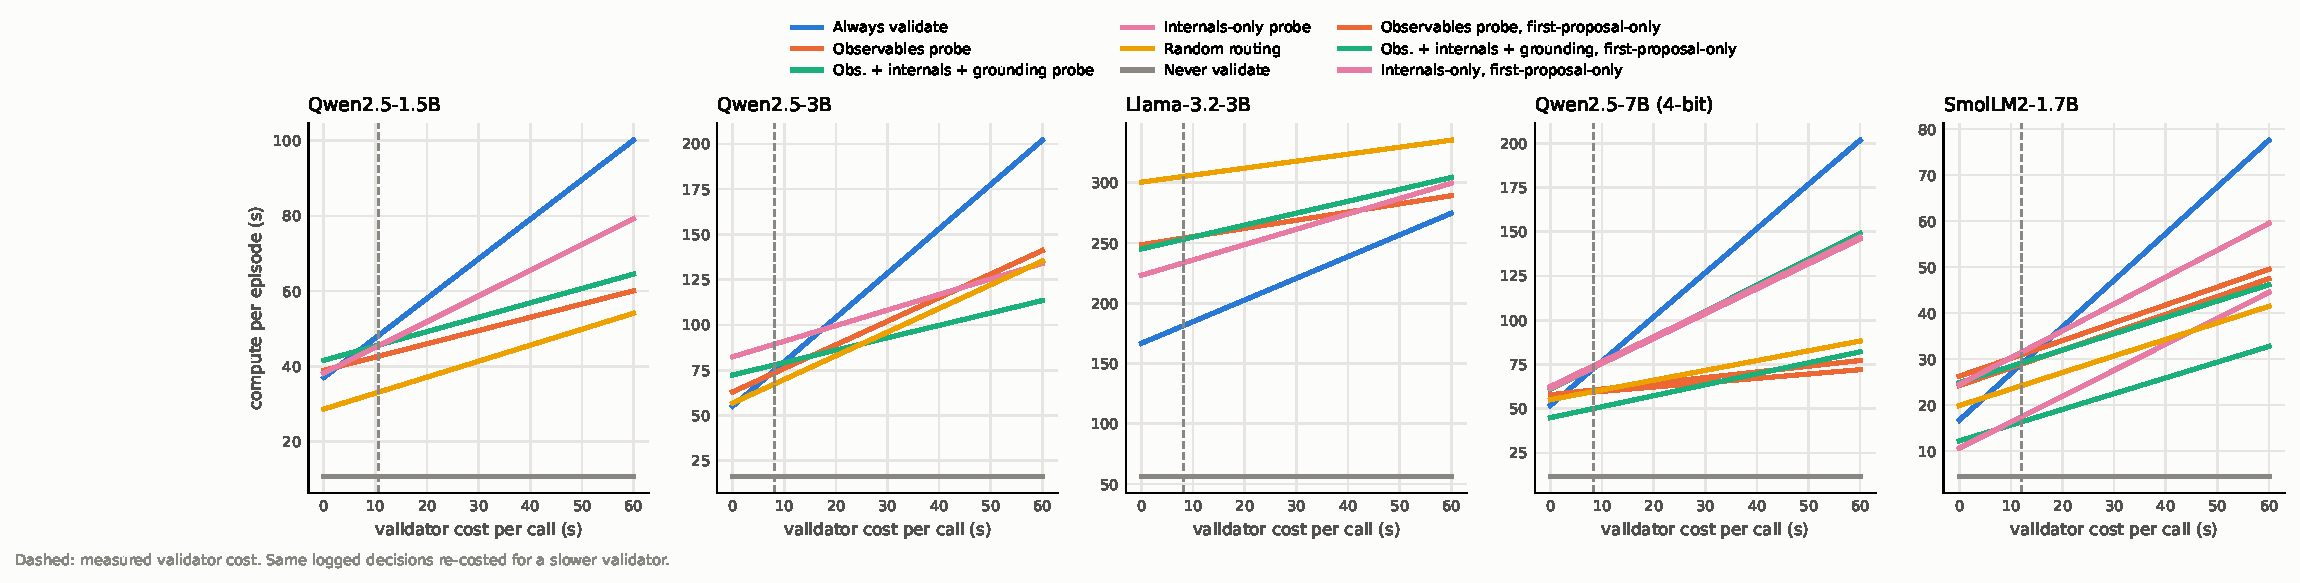
\includegraphics[width=\textwidth]{figures/closed_loop_compute_all.pdf}
\caption{Compute per closed-loop episode as a function of the validator's cost per call, for each model and policy.
The logged decisions are re-costed exactly; the dashed line marks the measured validator cost. Screens that avoid
validator calls overtake always-validate once validation costs more than a few seconds per call.}
\label{fig:costs}
\end{figure}
